\section{Methodology}

\subsection{Overview}

\begin{figure*}[t]
\centering
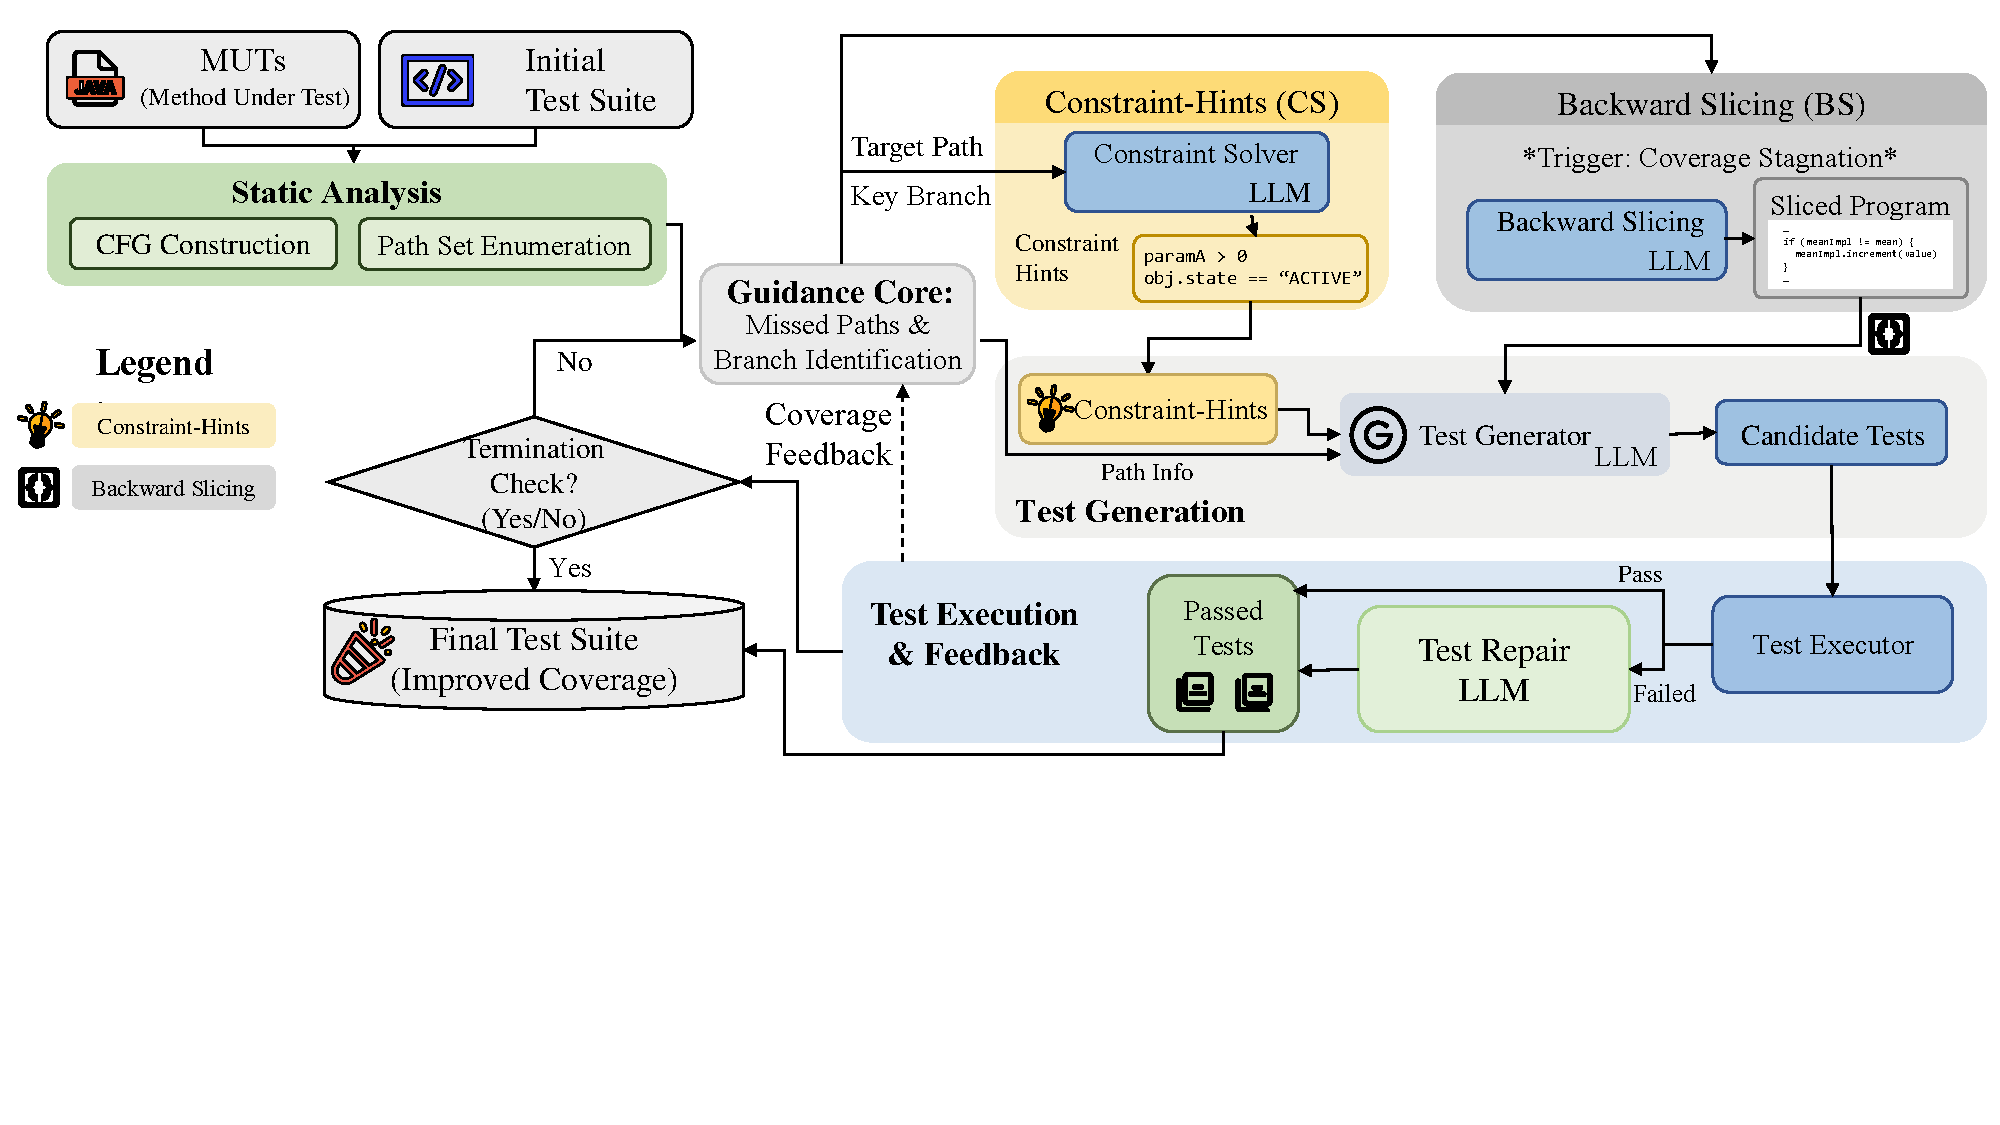
\includegraphics[width=\linewidth]{figures/overview.pdf}
\caption{Overview of the coverage-guided test generation framework.}
\label{fig:overview}
\end{figure*}

\ourmethod{} is a coverage-guided iterative framework for automated unit test generation, illustrated in Figure~\ref{fig:overview}.Given a method under test, \ourmethod{} first performs an initialization step that extracts project-level dependencies, resolves the required JUnit imports, and seeds the suite with a syntactically valid scaffolding test containing a trivial \texttt{assertTrue(true)} assertion, ensuring a compilable starting point for all subsequent iterations.It then constructs the CFG, enumerates feasible paths, and collects dynamic coverage feedback to identify uncovered branches before entering an iterative refinement loop.

Each iteration begins with path selection, where \textit{Constraint-Hints} analyzes the selected uncovered path and injects explicit branch conditions as structured guidance into the generation prompt.When coverage improvement stagnates, \textit{Backward Slicing} is activated, replacing the full method body with the minimal set of statements that bear data or control dependence on the target branch.The LLM then generates candidate tests against this focused context; passing tests are merged into the suite while failing ones are forwarded to the repair phase.During repair, compiler diagnostics—including error messages and their associated line numbers—are incorporated into the repair prompt, allowing the LLM to precisely locate and correct the offending statements rather than re-generating the test from scratch.Coverage is re-measured at the end of each iteration to drive target selection in the next round.The loop terminates when the coverage target is reached, the iteration budget is exhausted, or coverage fails to improve for a configurable number of consecutive iterations.

\subsection{Constraints-Hints}

\textit{Constraints-Hints} addresses the implicit precondition problem by 
decoupling constraint inference from test synthesis. Instead of requiring 
the LLM to simultaneously infer branch reachability and generate tests, 
we explicitly extract the conditions necessary to trigger a target branch 
and provide them as structured guidance.

While symbolic execution can derive precise path conditions, it often 
struggles to scale to real-world programs due to path explosion, complex 
heap interactions, and challenges in modeling external libraries and 
reflection~\cite{baldoni2018, cadar2008klee}. 
Rather than performing exact constraint solving, we aim to extract 
\emph{sufficient} conditions that characterize branch reachability.

Concretely, given an uncovered branch, we analyze its predicate and 
derive a set of constraint hints that describe the required program state 
(e.g., variable relations, nullness conditions, and key object properties). 
These hints are then embedded into the generation prompt, guiding the LLM 
to construct inputs and invocation sequences that satisfy the target condition.

By transforming implicit dependencies into explicit guidance, 
\textit{Constraints-Hints} reduces the reasoning burden on the LLM and 
enables more reliable generation of tests that reach previously uncovered branches.

\paragraph{Path formulation.}

Let $P = \langle b_1, b_2, \ldots, b_k \rangle$ denote the sequence of branch
decisions along a target execution path $\pi$, where each predicate
$b_i(\mathbf{x}) \in \{\texttt{true}, \texttt{false}\}$ is evaluated over the
program input vector $\mathbf{x}$. Covering the path requires an input
assignment $\mathbf{x}^*$ that satisfies all branch predicates along the
path:

\begin{equation}
\mathbf{x}^* \in \mathcal{F}(\pi) =
\left\{
\mathbf{x} \mid
b_1(\mathbf{x}) \wedge b_2(\mathbf{x}) \wedge \cdots \wedge b_k(\mathbf{x})
\right\}.
\end{equation}

Rather than solving this constraint system symbolically—which can be
computationally expensive and brittle under complex object states or
indirect method calls—\ourmethod{} employs an LLM-based constraint solver to
approximate the feasible input space as a lightweight set of interpretable conditions:

\begin{equation}
\mathcal{C}(\pi) =
\left\{
c_j \mid
c_j \text{ is a necessary condition on } \mathbf{x}
\right\}.
\end{equation}

The first uncovered branch along the path, denoted as $b^*$, is identified
from the coverage report and provided to the solver as additional context,
guiding the model toward the most immediate obstacle preventing the path
from being executed.

\paragraph{Integration.}

The constraint-solving prompt is generated from a configurable template that
incorporates the source code, the branch sequence of $\pi$, and the uncovered
branch $b^*$. The solver produces $\mathcal{C}(\pi)$ as a list of conditions
such as \texttt{paramA > 0} or \texttt{obj.status == "ACTIVE"}. These
conditions are appended to the test generation prompt, transforming an
opaque path coverage objective into a concrete specification of required
inputs.

\paragraph{Example.}

Consider the \texttt{addValue} method, which contains three conditional
branches dispatching to overridable statistical implementations. An
existing test suite covers only the false branches of all three predicates,
meaning \texttt{meanImpl}, \texttt{varianceImpl}, and \texttt{geoMeanImpl}
all refer to their default implementations. The first uncovered branch is
\texttt{(meanImpl != mean)}. The constraint solver identifies that
satisfying this predicate requires replacing the default implementation
before invoking \texttt{addValue}. This object-state precondition is
expressed as a constraint in $\mathcal{C}(\pi)$:

\[
c : \texttt{meanImpl} \neq \texttt{mean}
\]

which implies that a call such as \texttt{setMeanImpl(...)} must occur prior
to invoking \texttt{addValue}. By making this requirement explicit, the test
generation LLM can construct the correct setup sequence and cover the
previously unreachable branch.

\subsection{Backward Slicing}

Coverage improvement does not always progress smoothly: certain branches remain persistently uncovered even after multiple iterations, typically because their reachability depends on subtle state dependencies that standard generation fails to capture. 
When such a plateau is detected, \ourmethod{} triggers a backward slicing step targeted at these stubborn branches, replacing the full method body with the minimal context actually relevant to the uncovered path.

\paragraph{Slice extraction.}

Given an uncovered path $\pi$, the framework extracts the subset of statements that may influence the execution of that path:

\begin{equation}
\textit{Slice}(P,\pi) =
\left\{
s_i \in P \mid s_i \rightsquigarrow \pi
\right\}.
\end{equation}

A dedicated LLM is then invoked with the uncovered code segment, the focal method source code, and dependency context from related classes. The model returns a structured response containing the relevant slice statements, required input values, necessary object states, and potential setup operations.

\paragraph{Test generation from slices.}

The extracted slice information is supplied as additional context to the test generation prompt. The LLM then generates targeted unit tests that incorporate the identified prerequisites directly. These tests are compiled, executed, and measured using the same validation pipeline as regular test candidates, allowing the framework to recover from coverage plateaus while maintaining the overall iterative workflow.

\subsection{Iterative Workflow of \ourmethod{}}

\begin{algorithm}[t]
\small
\caption{Iterative Test Generation with Constraints-Hints and Backward Slicing}
\label{alg:main}
\SetAlgoLined
\KwIn{$\textit{src}$: source file, $\textit{suite}$: initial test suite (possibly empty)}
\KwOut{Augmented test suite with improved coverage}

$\textit{deps} \leftarrow \textsc{ExtractDeps}()$\;
$\textit{cfg}, \textit{methodDict} \leftarrow \textsc{BuildCFG}(\textit{src})$\;
$\textit{noIncr} \leftarrow 0$, \quad $\textit{iter} \leftarrow 0$\;
$\textit{cov}, \textit{missed} \leftarrow \textsc{RunCoverage}(\textit{suite})$\;

\While{$\textit{iter} < \textit{maxIter}$ \textbf{and} $\textit{noIncr} < \Lambda$ \textbf{and} $\textit{cov} < \tau$}{

    \tcp{Path selection and prompt construction}
    \eIf{$\textit{cov} = 0$ \textbf{or} $\textit{iter} = 0$}{
        $\textit{prompt} \leftarrow \textsc{BuildBaselinePrompt}(\textit{src}, \textit{suite}, \textit{deps})$\; \tcp*[r]{baseline prompt}
    }{
        $\Pi \leftarrow \textsc{SelectPaths}(\textit{cfg}, \textit{methodDict}, \textit{missed})$\;
        $\mathcal{C} \leftarrow \emptyset$\;
        \ForEach{path $\pi \in \Pi$}{
            $b^* \leftarrow \textsc{FirstUncoveredBranch}(\pi, \textit{missed})$\;
            $\mathcal{C}(\pi) \leftarrow \textsc{ConstraintSolver}(\textit{src}, \pi, b^*)$\; \tcp*[r]{Constraints-Hints}
        }
        $\textit{prompt} \leftarrow \textsc{BuildPrompt}(\textit{src}, \textit{suite}, \textit{deps}, \Pi, \mathcal{C})$\;
    }

    \tcp{Test generation}
    $\mathcal{T} \leftarrow \textsc{GenerateTests}(\textit{prompt})$\;

    \tcp{Backward slicing for stubborn uncovered paths}
    \If{$\textit{noIncr} \geq \beta \cdot \Lambda$}{
        $\textit{slices} \leftarrow \textsc{BackwardSlicer}(\textit{src}, \textit{missed})$\;
        $\mathcal{T} \leftarrow \mathcal{T} \cup \textsc{GenerateFromSlices}(\textit{slices}, \textit{suite}, \textit{deps})$\;
    }

    \tcp{Validation and repair}
    $\textit{failed} \leftarrow \{\}$\;
    \ForEach{$t \in \mathcal{T}$}{
        \lIf{$\textsc{ValidateTest}(t, \textit{suite})$}{$\textit{suite} \leftarrow \textit{suite} \cup \{t\}$}
        \lElse{$\textit{failed} \leftarrow \textit{failed} \cup \{t\}$}
    }
    \If{$\textit{failed} \neq \emptyset$}{
        $\textit{suite} \leftarrow \textit{suite} \cup \textsc{RepairAndValidate}(\textit{failed}, \textit{src}, \textit{suite}, \textit{deps})$\;
    }

    \tcp{Coverage update and termination check}
    $(\textit{cov}',\, \textit{missed}') \leftarrow \textsc{RunCoverage}(\textit{suite})$\;
    \lIf{$\textit{cov}' > \textit{cov}$}{$\textit{noIncr} \leftarrow 0$}
    \lElse{$\textit{noIncr} \leftarrow \textit{noIncr} + 1$}
    $\textit{cov} \leftarrow \textit{cov}'$, \quad
    $\textit{missed} \leftarrow \textit{missed}'$, \quad
    $\textit{iter} \leftarrow \textit{iter} + 1$\;
}

\Return $\textit{suite}$\;
\end{algorithm}

The complete workflow of \ourmethod{} is formalized in Algorithm~\ref{alg:main}. The framework accepts the source file and an initial test suite as input, and iteratively generates, validates, and repairs tests until a coverage target is met or a termination condition is triggered.


\paragraph{Initialization.}
The framework extracts test-scope dependencies, constructs the CFG and method dictionary from the source file, and measures baseline coverage on the initial suite (lines 1--4).

\paragraph{Path selection with Constraints-Hints.}
At each non-initial iteration, \textsc{SelectUncoveredPaths} identifies candidate paths from the CFG that intersect with missed lines or branches, weighted by both coverage impact and visit history $\textit{pathHistory}$ (line 8). For each selected path $\pi$, the constraint solver derives $\mathcal{C}(\pi)$ by analyzing the branch sequence up to the first uncovered predicate $b^*$, and these conditions are embedded into the generation prompt (lines 9--13).

\paragraph{Backward slicing.}
When $\textit{noIncr} \geq \beta \cdot \Lambda$, indicating a coverage plateau, the backward slicer is invoked on the remaining missed code segments. It returns structured prerequisite information---required inputs, object states, and method mocks---which is used to construct an additional batch of targeted tests $\mathcal{T}_s$ (lines 16--19).

\paragraph{Validation and repair.}
Each generated test is individually inserted into the suite and executed. Failing tests are collected with their error messages and forwarded to the repair phase, which re-invokes the LLM with failure feedback to produce corrected versions. Successfully validated repaired tests are also incorporated into the suite (lines 21--32).

\paragraph{Termination.}
The loop exits when the coverage target $\tau$ is reached, the maximum iteration count $\textit{maxIter}$ is exhausted, or coverage fails to improve for $\Lambda$ consecutive iterations.